\documentclass[aspectratio=169,11pt]{beamer}
\usepackage[utf8]{inputenc}\usepackage[spanish,es-nodecimaldot]{babel}
\usepackage{vh-beamer}\usepackage{newunicodechar}
\newunicodechar{ℝ}{\ensuremath{\mathbb{R}}}\newunicodechar{∧}{\ensuremath{\land}}
\newunicodechar{→}{\ensuremath{\to}}\newunicodechar{∃}{\ensuremath{\exists}}
\newunicodechar{∀}{\ensuremath{\forall}}\newunicodechar{≤}{\ensuremath{\le}}
\newunicodechar{⟨}{\ensuremath{\langle}}\newunicodechar{⟩}{\ensuremath{\rangle}}
\title[Verificación heterogénea y acceso a la IA]{Verificación heterogénea\\y acceso a la IA}
\subtitle{Presentación final --- Track A}
\author{Sofía Belén Vásquez García}\date{28 de octubre de 2026}
\begin{document}
\begin{frame}[plain]\titlepage
\begin{center}\small\href{https://github.com/sbvasquezg-ux/ai-project}{github.com/sbvasquezg-ux/ai-project}\end{center}
\end{frame}
\begin{frame}{La pregunta y el resultado}
\textbf{Pregunta:} ¿Puede un costo de validación decreciente desplazar el uso de IA desde la base hacia tipos intermedios?
\begin{block}{Resultado propio}
En una economía de tres tipos, bajo condiciones de ofertas netas y suficiente masa experta, existe un equilibrio único donde \textbf{solo adopta el tipo intermedio}.
\end{block}
\begin{itemize}
\item Prueba completa del régimen discreto.
\item Equilibrio sobre mallas uniformes: evidencia numérica de adopción intermedia.
\item El continuo sigue abierto como resultado general.
\end{itemize}
\end{frame}
\begin{frame}{Baseline y supuesto modificado}
\textbf{Ide y Talamàs (2025), Proposición 6, p. 27 de arXiv v11.}
\begin{itemize}
\item IA no autónoma: solo asesora.
\item Con adopción, usuarios en la base y salario $w^N=a$ entre usuarios.
\item El beneficio no incorpora un gasto real de validación por tipo.
\end{itemize}
\medskip
\textbf{Extensión:} $c(z)=\kappa(1-z)$, $\kappa\geq0$, en bien final por trabajador y período.
\begin{keybox}
El modelo conserva tiempo y probabilidad de éxito. El aporte es la selección competitiva con esta fricción.
\end{keybox}
\sourcefoot{Paper base, secciones 3.1 y 6; antecedentes: Xu et al., Quispe--Xu, Catalini et al.}
\end{frame}
\begin{frame}{Primitivas y actividades}
\begin{columns}[T]
\column{.53\linewidth}
\begin{itemize}
\item $z$: conocimiento humano; $a$: capacidad de la IA.
\item $h$: tiempo de ayuda por consulta.
\item $b(z)=h(1-z)$; $n(z)=1/b(z)$.
\item $\mu>h$: cómputo ocioso y $r=0$.
\end{itemize}
\column{.43\linewidth}
\textbf{Tres actividades}\par\medskip
Independiente: produce $z$.\par\medskip
Humano--humano: trabajador $z$, solver $s>z$.\par\medskip
Humano--IA: producto neto $q(z)=a-c(z)$, si $z\leq a$.
\end{columns}
\medskip
Tipos observables, competencia, libre entrada y dos niveles.
\end{frame}
\begin{frame}{Asignación y precios de equilibrio}
\small
$d_i$: independientes; $x_i$: usuarios IA; $y_{ij}$: trabajadores $i$ ayudados por humanos $j$.
\[
\max_{d,x,y\geq0}\ \sum_i z_id_i+\sum_{z_i\leq a}q_ix_i+\sum_{i<j}z_jy_{ij}
\]
\[
d_i+x_i+\sum_{j>i}y_{ij}+\sum_{k<i}h(1-z_k)y_{ki}=M_i.
\]
\textbf{No beneficio positivo:}
\[
w_i\geq z_i,\qquad w_i\geq q_i\ (z_i\leq a),\qquad
w_i+h(1-z_i)w_j\geq z_j.
\]
Igualdad en actividades utilizadas. Las variables primales $x_i$ identifican usuarios; la igualdad $w_i=q_i$ puede indicar solo indiferencia.
\end{frame}
\begin{frame}{Proposición 1: condición local}
\[
\Pi^V(z)=n(z)[a-w^V(z)-c(z)]-r,\quad 0\leq z\leq a.
\]
Si $0<z<a<1$, $h>0$, $w^V,c$ son diferenciables y hay un máximo local:
\[
w^{V\prime}(z)+c'(z)=\frac{a-w^V(z)-c(z)}{1-z}.
\]
\begin{block}{Actividad usada y cómputo ocioso}
Con beneficio cero y $r=0$, $w^V(z)=a-c(z)$.\par
En un intervalo activo diferenciable, $w^{V\prime}(z)=\kappa$.
\end{block}
\alert{Esta proposición no identifica el conjunto de usuarios.}
\end{frame}
\begin{frame}{Proposición 2: condiciones del régimen intermedio}
\small
Tipos $(0,m,H)$, $0<m<H<1$, masas $(\alpha,\beta,\gamma)>0$, suma uno, $m<a$. Defino
\[
 b_M=h(1-m),\quad v_L=H(1-h),\quad v_M=H(1-b_M).
\]
\textbf{Condiciones suficientes:}
\begin{align*}
\gamma&>h\alpha+b_M\beta &&\text{expertos excedentes},\\
v_M&>m &&\text{alternativa humana de }M,\\
q_L&<v_L,\qquad q_M>v_M &&\text{base y medio},\\
q_H&<H\quad\text{si }H\leq a &&\text{expertos no adoptan}.
\end{align*}
Entonces hay equilibrio único con $w^V=(v_L,q_M,H)$ y usuarios IA $(0,\beta,0)$.
\sourcefoot{Resultado propio, especialización discreta del modelo. No es un teorema del continuo.}
\end{frame}
\begin{frame}{Prueba local: regla del producto}
\[
n(z)=\frac{1}{h(1-z)},\quad n'(z)=\frac{1}{h(1-z)^2},\quad\frac{n'}n=\frac1{1-z}.
\]
\[
0=\underbrace{n'(z)[a-w^V-c]}_{\text{cambio en escala}}
-\underbrace{n(z)[w^{V\prime}+c']}_{\text{cambio en costo por trabajador}}.
\]
\begin{itemize}
\item Se mantienen fijos $a,h,r$ al derivar respecto de $z$.
\item La interioridad permite aplicar Fermat; $n>0$ permite dividir.
\item En extremos corresponden desigualdades unilaterales.
\end{itemize}
\end{frame}
\begin{frame}{Beneficio cero y pendiente salarial}
\[
n(z)[a-w^V(z)-c(z)]=r
\ \Longrightarrow\ a-w^V(z)-c(z)=rh(1-z).
\]
\[
w^{V\prime}+c'=hr;\qquad r=0\ \Longrightarrow\ w^V=a-c.
\]
\textbf{Con costo lineal:}
\[
w^V=a-\kappa+\kappa z,\quad w^{V\prime}=\kappa.
\]
\begin{keybox}
La igualdad salarial procede de beneficio cero. La FOC es otra condición; por sí sola no determina la asignación.
\end{keybox}
\end{frame}
\begin{frame}{Prueba del equilibrio: construir la asignación}
\begin{center}
\begin{tabular}{lll}\toprule
Tipo & Actividad & Masa\\\midrule
$L$ & Trabajador con experto $H$ & $\alpha$\\
$M$ & Usuario de IA & $\beta$\\
$H$ & Solver de $L$ & $h\alpha$\\
$H$ & Independiente & $\gamma-h\alpha$\\\bottomrule
\end{tabular}
\end{center}
\[
(w_L,w_M,w_H)=(v_L,q_M,H).
\]
Las masas se vacían. La demanda de cómputo $b_M\beta<h<\mu$ deja $r=0$.
\medskip
Sin IA, $M$ también trabajaba con $H$; había $\gamma-h\alpha-b_M\beta>0$ expertos independientes.
\end{frame}
\begin{frame}{Prueba del equilibrio: revisar los desvíos}
\small
\begin{tabular}{lll}\toprule
Actividad & Holgura salarial & Resultado\\\midrule
$LH$ & $v_L+hH-H=0$ & Usada\\
IA de $M$ & $w_M-q_M=0$ & Usada\\
Independiente $H$ & $w_H-H=0$ & Usada\\
$MH$ & $q_M-v_M>0$ & No usada\\
$LM$ & $v_L+hq_M-m>0$ & No usada\\
IA de $L$ & $v_L-q_L>0$ & No usada\\
IA de $H$, si elegible & $H-q_H>0$ & No usada\\\bottomrule
\end{tabular}\par
\medskip
Los tipos $L,M$ tampoco producen solos: $v_L>0$, $q_M>v_M>m$.
\[
v_L+hv_M-m=(v_M-m)+Hh(1-h)(1-m)>0.
\]
Como $q_M>v_M$, la holgura $LM$ también es positiva.
\end{frame}
\begin{frame}{Prueba de unicidad y ganancia neta}
\begin{enumerate}
\item Los precios candidatos acotan el producto de toda asignación factible.
\item La asignación construida alcanza la cota: es óptima.
\item Toda asignación óptima usa solo actividades de holgura cero.
\item Recursos fijan sus masas; beneficio cero fija los tres salarios.
\end{enumerate}
\medskip
\[
Y^V-Y^0=\beta[q_M-H(1-b_M)]
=\beta(q_M-v_M)>0.
\]
El resultado usa todas las alternativas y el vaciado del mercado. No se obtiene sustituyendo salarios iniciales en la FOC.
\end{frame}
\begin{frame}{Ejemplo exacto de tres tipos}
\small
$h=0.5$, $a=0.88$, $\kappa=0.53$; $z=(0,0.25,0.76)$; masas $(0.25,0.40,0.35)$.
\begin{center}
\begin{tabular}{rrrrr}\toprule
$z$ & $w^0$ & $q(z)$ & $w^V$ & Masa con IA\\\midrule
0.00&0.3800&0.3500&0.3800&0.00\\
0.25&0.4750&0.4825&0.4825&0.40\\
0.76&0.7600&0.7528&0.7600&0.00\\\bottomrule
\end{tabular}
\end{center}
\[
Y^0=0.551,\qquad Y^V=0.554,\qquad\Delta Y=0.003.
\]
\begin{itemize}
\item Solo $M$ usa IA; la base conserva su salario.
\item Certificado racional exacto y LP independiente coinciden.
\item Los parámetros son ilustrativos, sin calibración empírica.
\end{itemize}
\sourcefoot{code/output/three\_type.csv; prueba propia en el paper. Distribución distinta de la ilustración inicial uniforme.}
\end{frame}
\begin{frame}{Simulación del continuo: salarios y usuarios}
\centering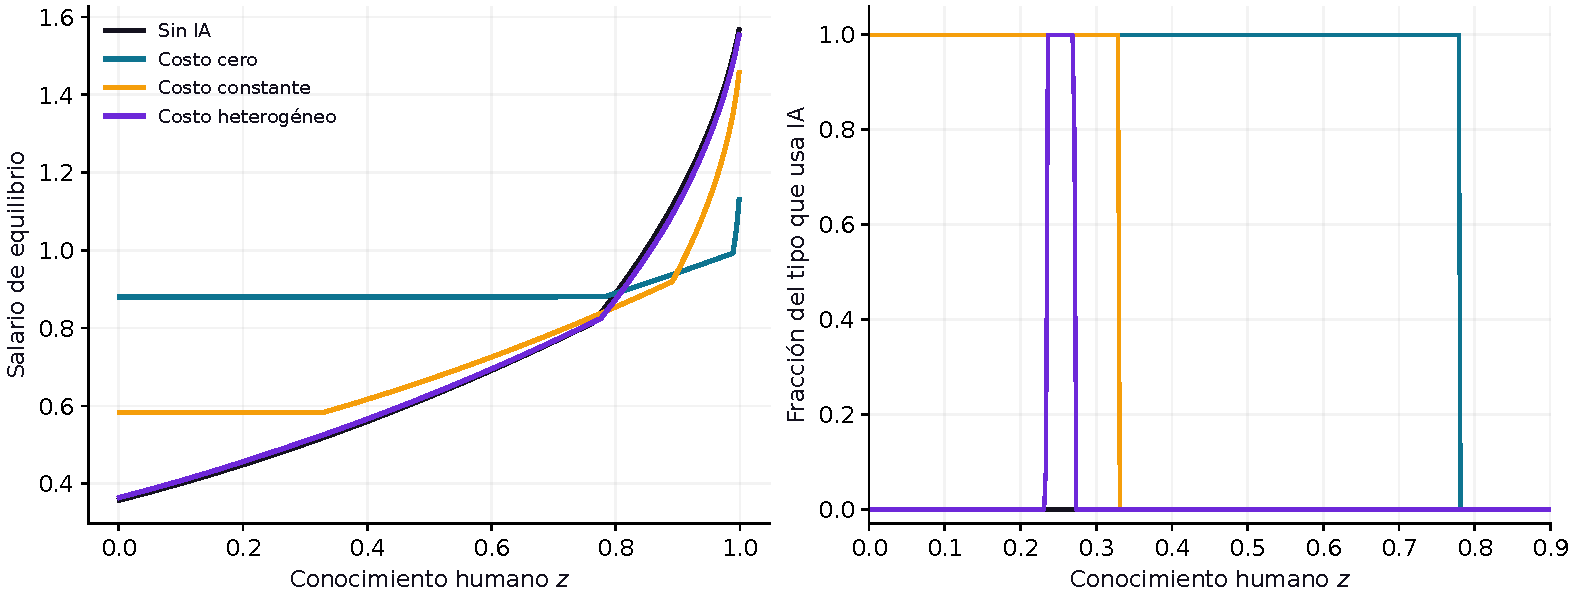
\includegraphics[width=.98\linewidth]{../code/figures/equilibrium.pdf}
\small
$G(z)=z$, $h=.5$, $a=.88$, $\kappa=.53$, $N=400$.\par
Costo constante: $\bar c=\kappa(1-a/2)=.2968$, promedio entre elegibles.
\sourcefoot{Cálculo propio con primal y dual. El gasto realizado no se iguala entre escenarios.}
\end{frame}
\begin{frame}{Sensibilidad a la malla y límites}
\begin{center}\small
\begin{tabular}{rrrrr}\toprule
$N$ & Producto neto & Masa IA & Mínimo $z$ & Máximo $z$\\\midrule
100&0.692416&0.042187&0.23500&0.27500\\
200&0.692471&0.033137&0.23750&0.27250\\
400&0.692483&0.037226&0.23375&0.27125\\\bottomrule
\end{tabular}\end{center}
\begin{itemize}
\item Recursos, beneficios, complementariedad y brecha primal--dual: residuos $<10^{-7}$.
\item El patrón intermedio persiste en las tres mallas.
\item Las masas oscilan: no se afirma convergencia ni unicidad del continuo.
\item El gasto heterogéneo no domina al constante en producto neto.
\end{itemize}
\end{frame}
\begin{frame}[fragile]{Lean: existencia y unicidad del mismo equilibrio}
\small
\textbf{En el paper:} bajo las condiciones de la Proposición 2, existe un único equilibrio en asignaciones y salarios, con y sin IA.
\medskip\par
\textbf{En Lean, parte con IA de \texttt{PropositionTwoSpec}:}
\begin{footnotesize}\begin{verbatim}
Equilibrium e true (candidateAllocation e true)
  (candidatePrices e true) ∧
∀ x p, Equilibrium e true x p →
  x = candidateAllocation e true ∧ p = candidatePrices e true
\end{verbatim}\end{footnotesize}
\textbf{Fragmento que prueba esa conjunción:}
\begin{footnotesize}\begin{verbatim}
exact ⟨candidate_equilibrium e true hr,
       equilibrium_unique e true hr⟩
\end{verbatim}\end{footnotesize}
\texttt{hr} reúne las condiciones primitivas de la Proposición 2. El enunciado completo prueba también el baseline, $r=0$ y la ganancia neta.\par
\textbf{Qué verifica:} las nueve actividades, recursos, elegibilidad y unicidad; no se supone que el candidato ya sea equilibrio.
\end{frame}
\begin{frame}{Una restricción que introdujo la IA}
\textbf{Borrador anterior:} impuso $0\leq\kappa<1$ al costo lineal.
\[
z\in[0,1],\quad\kappa\geq0
\ \Longrightarrow\ c(z)=\kappa(1-z)\geq0.
\]
La no negatividad del gasto no exige $\kappa<1$. Costos altos pueden excluir actividades sin invalidar la definición de la tecnología.
\begin{keybox}
Veredicto del chequeo del asistente: la cota superior era injustificada.\par
La autora debe reconstruir la prueba y confirmar su propio veredicto.
\end{keybox}
\small\medskip
Manuscrito de la autora pendiente: incorporar una fotografía real antes de exponer. Guía: \texttt{hand/guia-derivaciones.pdf}.
\end{frame}
\begin{frame}{Resultados demostrados y trabajo abierto}
\begin{columns}[T]
\column{.48\linewidth}
\textbf{Demostrado y formalizado}
\begin{itemize}
\item Relación local de salarios.
\item Equilibrio único en el régimen de tres tipos.
\item Ganancia neta en ese régimen.
\end{itemize}
\column{.48\linewidth}
\textbf{Abierto}
\begin{itemize}
\item Caracterización global del continuo.
\item Convergencia de asignaciones.
\item Revisión manuscrita humana.
\end{itemize}
\end{columns}
\medskip
La extensión es propia. Las limitaciones delimitan el resultado y no atribuyen un error a Ide y Talamàs.
\end{frame}
\begin{frame}{Preguntas para la discusión}
\begin{enumerate}
\item ¿El gasto real por trabajador aísla un mecanismo útil de acceso, o conviene extender luego a tiempo de validación?
\item ¿Qué condiciones permitirían trasladar el certificado de tres tipos a una distribución continua?
\item ¿Qué comparación de costos resulta más informativa: igual promedio entre elegibles o igual gasto realizado?
\end{enumerate}
\medskip
\href{https://github.com/sbvasquezg-ux/ai-project}{github.com/sbvasquezg-ux/ai-project}
\end{frame}
\appendix
\begin{frame}{A. Entrada a salarios iniciales}
\centering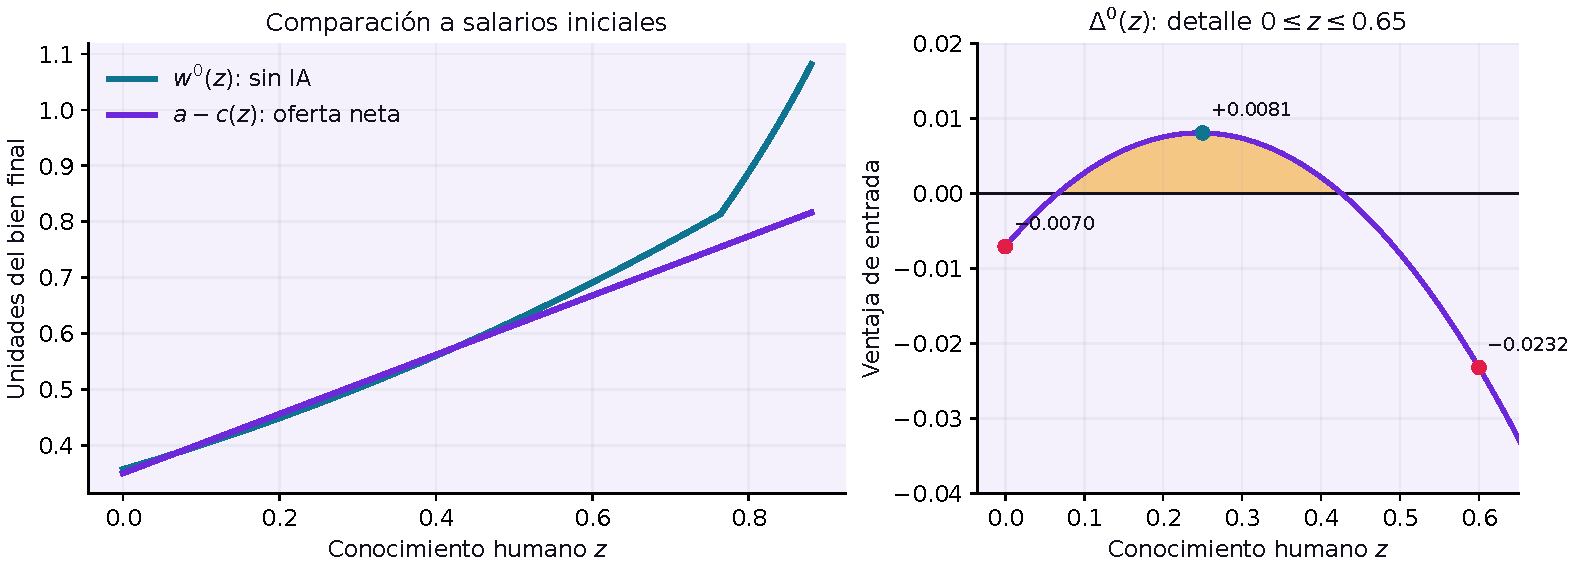
\includegraphics[width=.93\linewidth]{../code/figures/entry_check.pdf}\par
\small La ilustración del topic sigue siendo una comparación de entrada. Los salarios del nuevo equilibrio se obtienen por separado.
\end{frame}
\begin{frame}{B. Costo cero y constante}
\small
Con $c=0$ se recuperan las actividades del baseline y la oferta $q=a$.
\[
 c(z)=\bar c\Rightarrow q'=0,\qquad c(z)=\kappa(1-z)\Rightarrow q'=\kappa.
\]
En la malla de 400 tipos:
\begin{center}\begin{tabular}{lrr}\toprule
Escenario & Producto neto & Masa IA\\\midrule
Sin IA&0.692334&0.000000\\
Costo cero&0.893418&0.780000\\
Costo constante&0.729923&0.330000\\
Costo heterogéneo&0.692483&0.037226\\\bottomrule
\end{tabular}\end{center}
No se modela el daño de una validación omitida; no es una evaluación de una política regulatoria.
\end{frame}
\begin{frame}{C. Referencias y reproducción}
\footnotesize
\begin{itemize}
\item Ide y Talamàs (2025), JPE 133(12), 3762--3800. \href{https://doi.org/10.1086/737233}{DOI}; \href{https://arxiv.org/abs/2312.05481v11}{arXiv v11}, Prop. 6, p.27.
\item \href{https://www.eduardtalamas.com/}{Online Appendix}, sección 2.6 y capítulo 5.
\item Xu et al., \href{https://arxiv.org/abs/2506.00532v2}{arXiv:2506.00532v2}, 2026; preprint.
\item Quispe y Xu, \href{https://arxiv.org/abs/2605.25438v2}{arXiv:2605.25438v2}, 2026; preprint.
\item Catalini et al., \href{https://arxiv.org/abs/2602.20946}{Some Simple Economics of AGI}, 2026; preprint.
\end{itemize}
\medskip
\texttt{python3 code/verify.py}: tabla inicial, ejemplo exacto, equilibrios y figuras.\par
Pruebas completas y bibliografía: \texttt{paper/paper.pdf}.\par
Guía de estudio: \texttt{hand/guia-derivaciones.pdf}.
\end{frame}
\end{document}
